\section{Auswertung}
Um zu verstehen, welchen Einfluss die Signallaufzeiten in der Schaltung haben,
wurde die Verzögerung dar Signale, die von den beiden zu SC2 gehörenden
Photomultipliern PM2 und PM4 ausgehen, mit einem Oszilloskop gemessen. Dabei
erhielten wir Bilder wie das in \fref{koinzidenz} dargestellte.

\begin{figure}[htb]
   \centering
   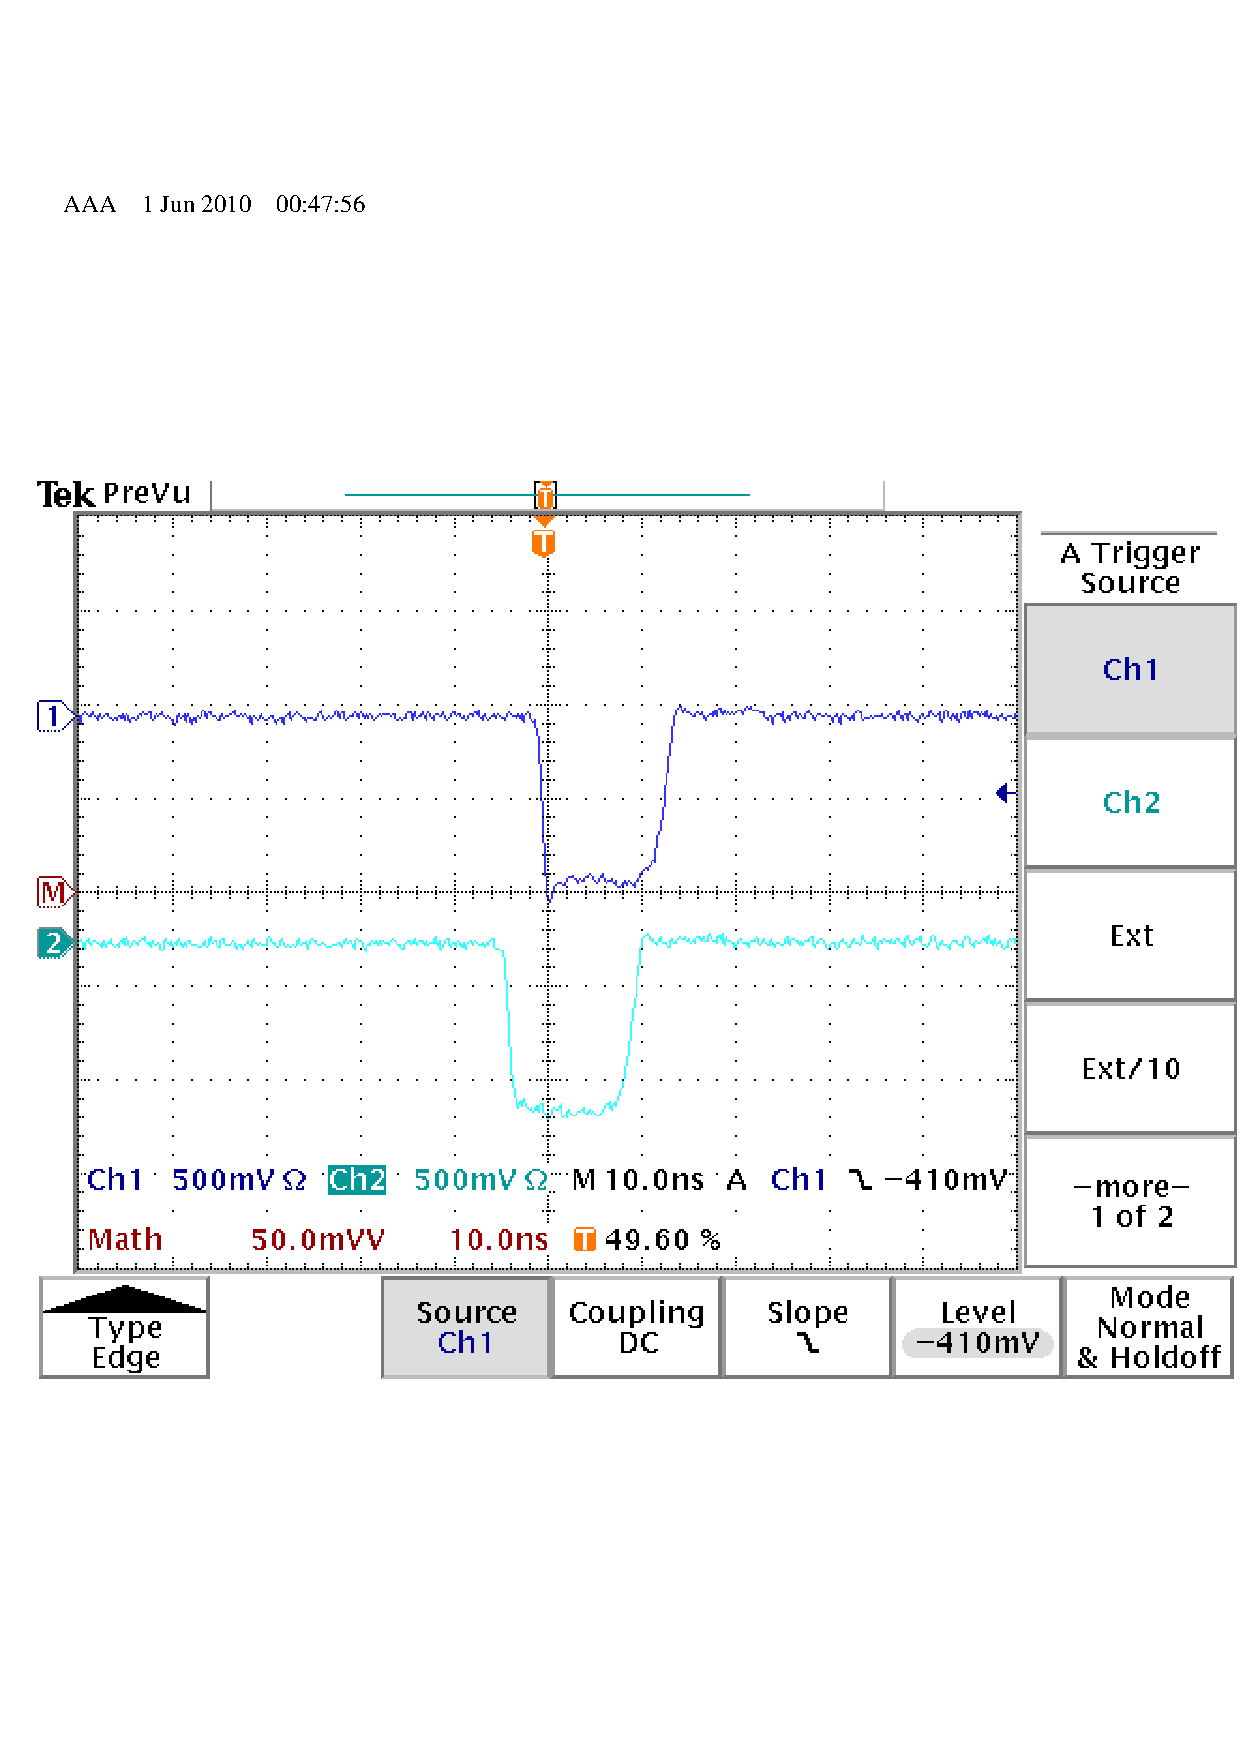
\includegraphics[width=1\columnwidth,keepaspectratio]{../data/TEK00000.pdf}
   \caption{Verzögerung in einer Koinzidenzeinheit}
   \label{fig:koinzidenz}
\end{figure}